\documentclass[twocolumn]{ctexart}

\usepackage{amsmath}
\usepackage{graphicx}
\begin{document}
\title{情感分析算法实验报告}
\author{ZF1921517 谢俊 ZF921239 王子扩 ZF1921333 刘冀星 ZF1921435 王德强}
\date{\today}
\maketitle

% \tableofcontents


\begin{abstract}
随着各种社交平台的兴起,网络上用户的生成内容越来越多,产生大量的文本信息,如新闻、微博、博客等,面对如此庞大且富有情绪表达的文本信息,完全可以考虑通过探索他们潜在的价值为人们服务。本实验是目标是实现对新闻文本进行分类,情感倾向分为三类,其中正面情绪为对应0,中性情绪对应1以及负面情绪对应2
\end{abstract}


\section{数据集介绍}

本实验使用的数据集是CCF大数据与计算智能大赛官网公开的数据集。数据集采用的互联网线上数据,数据爬取网站包括新闻网、微信、博客、贴吧等。
数据集为.CSV格式文件,分为训练集、验证集以及测试集。每个文件有四个项目,分别是新闻ID、新闻标题、新闻正文内容、新闻情感标签,格式如下:
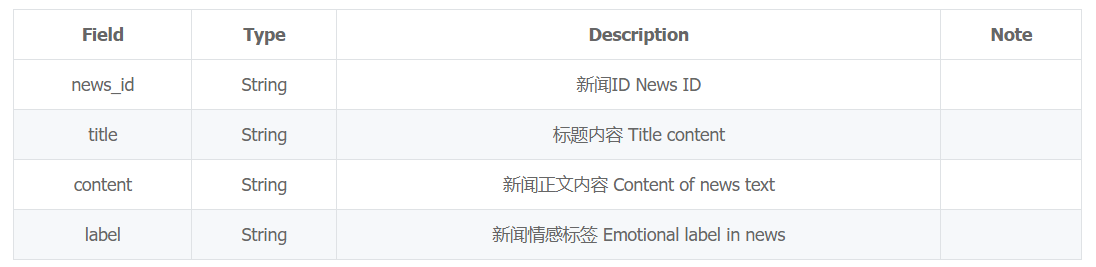
\includegraphics[width=0.5\textwidth]{p1.png}


\section{数据预处理}
由于训练数据集的内容和标签的数据集中id字段不一致、三个数据集存在较多标点符号和无用符号、存在停用词、存在title和content字段分开等问题,所以在预处理阶段所做的主要工作有:提取共有的内容、清理数据集的标点符号和英文字符、对数据集进行分词、去停用词、合并title和content字段。
\par 训练集结构结构展示如下图所示:\\
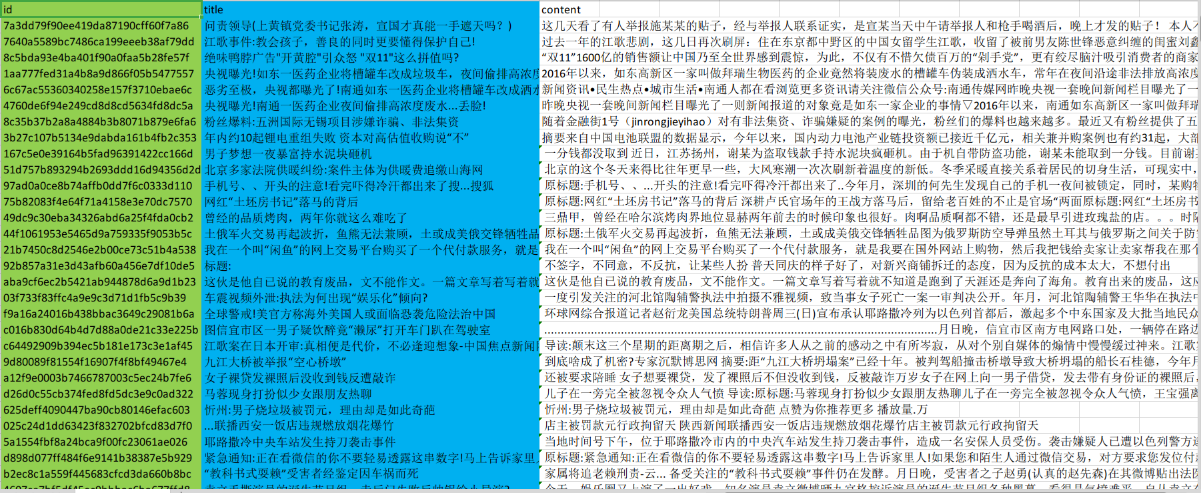
\includegraphics[width=0.5\textwidth]{p2.png}

\subsection{数据清洗}
\par 文本中包含很多无意义的特殊字符,如HTML标签、URL标点符号等,这类字符会影响词向量的生成,并且不会对文本的理解有帮助,因此需要将这些字符去除。

\par 本实验清洗特殊字符使用的正则表达式方式,主要使用了sub函数来删除想要去掉的字符。

\subsection{分词}
\par 本实验使用的是中文数据集。对于中文文本来说,词是以字为基本单位的,一篇文章的语义表达却可以用有序的词来表达。在处理中文文本时,需要进行分词处理,即将句子转化为词的表达。
\par 中文分词具有代表性的算法有正向最大匹配法(Maximum Match Method, MM 法)、逆向最大匹配法(Reverse Match Method, RMM 法)、双向最大匹配法(Bi-direction Matching Method)。
\par “Jieba”中文分词目前在中文文本分词中应用比较广泛,也有比较好的效果,因此本实验使用的“Jieba”分词工具。

\subsection{去停用词}
\par 停用词一般指人类语言中包含的功能词,这些功能词极其普遍,如:“是”、“你”、“而”、“故”等。与其他词相比,这类词没有实际的含义。另外还有些词频繁出现在文本中,由于频繁出现,我们可以认为这类词对文本的定位起不到实质性的作用。

\par 总之停用词对文本的分类起不到作用,并且会增加整个模型的运行负担,因此需要去除。本实验使用的是哈工大的停用词表,即,新闻文本中出现了停用词表中的词汇,就进行去除操作。

\subsection{词嵌入}
\par 词嵌入向量(Word Embedding)是NLP里面一个重要的概念,我们可以利用Word Embedding将一个单词转换成固定长度的向量表示,从而便于进行数学处理。One-hot编码是最为简单的获取词向量的方式,但这种既需要极大的空间用于存储,也不能从词向量中获得有用的词之间的语义关系,因此效果较差。

\par Word2Vec是一种结合上下文的词嵌入方式。由于 Word2vec 会考虑上下文,跟之前的词嵌入方法相比,效果要更好。而且维度更少,所以速度更快。并且这种方法通用性很强。因此本实验使用Word2Vec的方法来获取词向量。

\section{网络模型LSTM}
\par 长短期记忆网络(long-short term memory) - 通常称为“LSTM” - 是一种特殊的RNN,能够学习长期的规律。 它们是由Hochreiter与Schmidhuber(1997)首先提出的,并且在后来的工作中被许多人精炼和推广。他们在各种各样的问题上应用得非常好,现在被广泛的使用。

\par LSTM明确旨在避免长期依赖性的问题。 长时间记住信息实际上是他们的默认行为,而不是他们难以学习的东西。

\par 所有递归神经网络都具有神经网络重复模块链的形式。 在标准RNN中,该重复模块将具有非常简单的结构,例如单个tanh层。

\par LSTM也具有这种类似链的结构,但重复模块具有不同的结构,如下图所示。
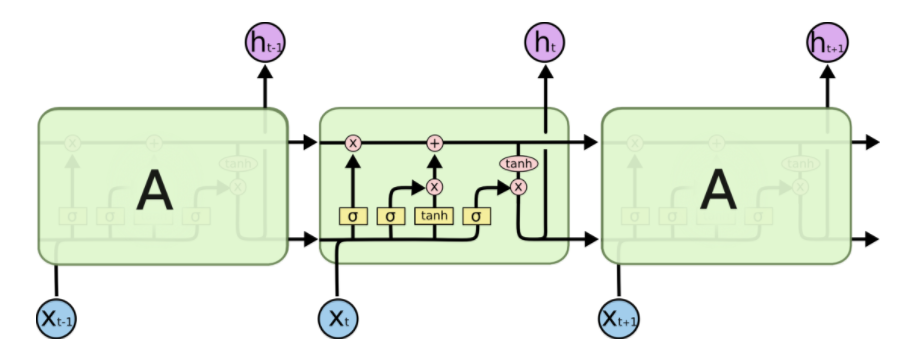
\includegraphics[width=0.5\textwidth]{p3.png}

\par 在上图中,每箭头都携带一个向量,从上一个节点的输出到其他节点的输入。 粉色圆圈表示逐点运算,如矢量加法,而黄色框表示神经网络层。 箭头合并表示连接,而箭头分叉表示其内容被复制,副本将转移到不同的位置。




\section{训练与预测}
本文提出的模型主要解决了对高昂的短语级注释的代价,同时也通过结果证明了情感词、否定词、强度词在情感分析中的作用。本文的模型采用的是序列LSTM,不依赖于解析树结构,是为了保持模型的简单性。在后续研究中作者也会将语言正则化应用于Tree-LSTM解决范围问题,因为解析数更容易明确的指示修改范围。
\subsection{模型训练阶段}
\par 1、

设置LSTM模型的初始化参数,包括:网络的隐藏层数hiddenSize、学习率learningRate, LSTM结构层数layer、训练数据大小batchSize、训练数据截取长度step、训练的轮数epoch、节点dropout的概率keepProb、优化器衰减系数WEIGHT_DECAY等;
\par 2、
提取出经由CBOW模型训练生成的词向量集合W中包含的训练样本集中所有词的词向量,并生成词向量集合Trn ={X0、X1、X2、……Xn};

\par 3、
将训练生成的词向量集合输入到LSTM层,通过LSTM单元结构生成表达词向量集H={H0、H1、H2、……Hn};
\par 4、
将经LSTM层生成的词向量集H作为平均池化层的输入,生成表达词向量;
\par 5、
将输入逻辑回归层,最后生成输入样本的情感标签;
\par 6、
定义损失函数,通过迭代使用反向传播算法不断调整模型的参数及样本输入的词向量;
\par 7、
生成LSTM情感分析摸并将训练好的模型参数导出;
\subsection{损失函数}
熵是表示随机变量不确定性的度量,是对所有可能发生的时间产生的信息量的期望。公式如下:
\begin{equation}
H(x) = -\sum_{i=1}^{n}p(x)log(p(x))
\end{equation}



\par 相对熵又称KL散度,用于衡量对于同一个随机变量x的两个分部p(x)和q(x)之间的差异。KL散度的公式如下:
\begin{equation}
D_{KL}(p||q)=-\sum_{i=1}^{n}p(x_i)log(\frac{p(x_i)}{q(x_i)})
\end{equation}
\par 将KL散度的公式进行变形得到:
\begin{equation}
D_{KL}(p||q)=-H(p(x))+[-\sum_{i=1}^{n}p(x_i)log(q(x_i))]
\end{equation}

\par 我们常常用KL散度来评估预测值与真实值之间的差别,因为KL散度前半部分是一个常量所以将后半部分交叉熵作为损失函数。交叉熵公式如下:
\begin{equation}
H(p,q)=-\sum_{i=1}^{n}p(x_i)log(q(x_i))]
\end{equation}
\par 在用梯度下降法做参数更新的时候,模型学习的速度取决于两个值:一、学习率;二、偏导值。其中,学习率是我们需要设置的超参数,所以我们重点关注偏导值。偏导值的大小取决于xi和 σ(s)-y ,后者的大小值反映了模型的错误程度,该值越大,说明模型效果越差,但是该值越大同时也会使得偏导值越大,从而模型学习速度更快。所以,使用逻辑函数得到概率,并结合交叉熵当损失函数时,在模型效果差的时候学习速度比较快,在模型效果好的时候学习速度变慢。但是这种方法也有一些缺点,softmax+cross-entropy loss 擅长于学习类间的信息,因为它采用了类间竞争机制,它只关心对于正确标签预测概率的准确性,忽略了其他非正确标签的差异,导致学习到的特征比较散。基于这个问题有很多优化,比如对softmax进行改进,如L-Softmax、SM-Softmax、AM-Softmax等。

\subsection{预测过程}
\par 1、
提取出词向量集合W中所包含的测试样本集中所有词向量,并生成词向量集合Tst={w0、w1、w2、……wn};
\par 2、
类似进行模型训练阶段中的步骤(3)、(4)、(5)的操作,最后生成测试样本的情感标签;
\par 3、
输出结果。
\par 4、为评价本文所提出的情感分析模型,我们采用准确率(Accuracy)作为评价标准。模型对新闻情绪进行分类,0代表正面情绪、1代表中性情绪、2代表负面情绪。

准确率:\begin{equation}
Accuracy=\frac{T_{pos}+T_{neu}+T_{neg}}{D_{test}}
\end{equation}

\section{实验结果}
\subsection{调参结果}
\par 实验过程主要调整的参数是Dropout的比例、隐藏层的数量、训练次数。
以下是实验过程中尝试几组参数的结果:
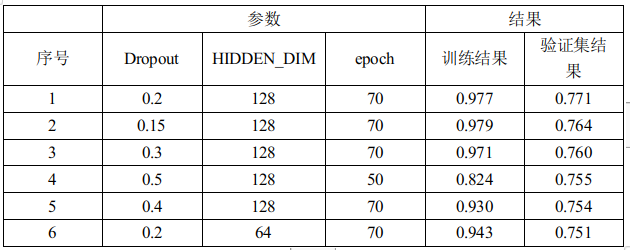
\includegraphics[width=0.5\textwidth]{p10.png}
\par 由此可见,当Dropout为0.2,隐藏层数量为128,训练次数为70时效果训练集与验证集的效果最好。
\par 以下是训练过程中的准确率曲线:
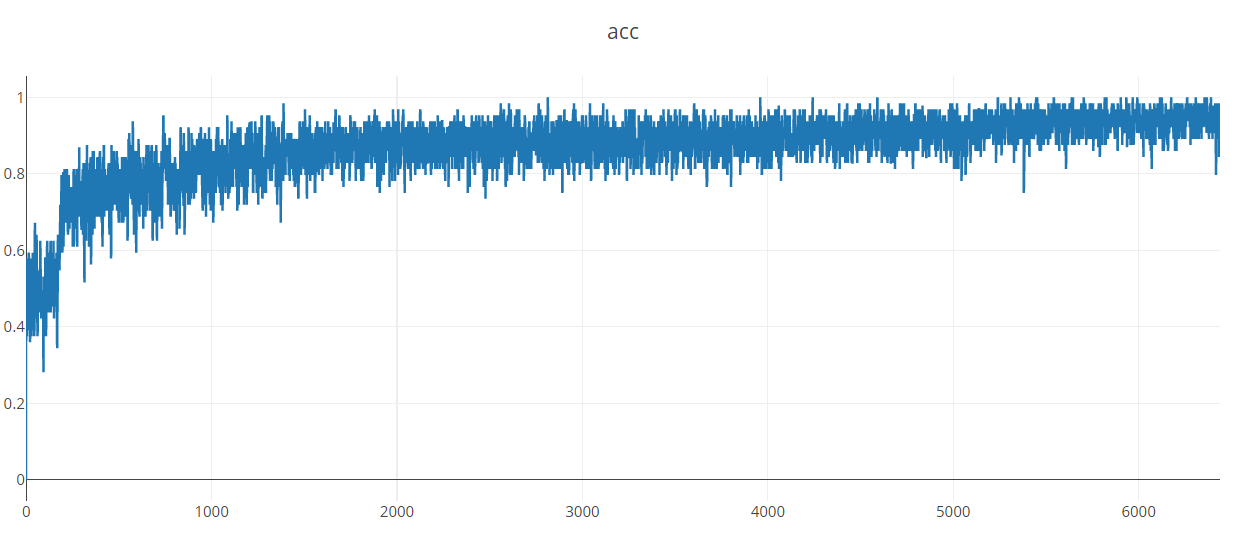
\includegraphics[width=0.5\textwidth]{p11.png}

\subsection{LOSS曲线}
\par 以下是训练过程中的loss曲线
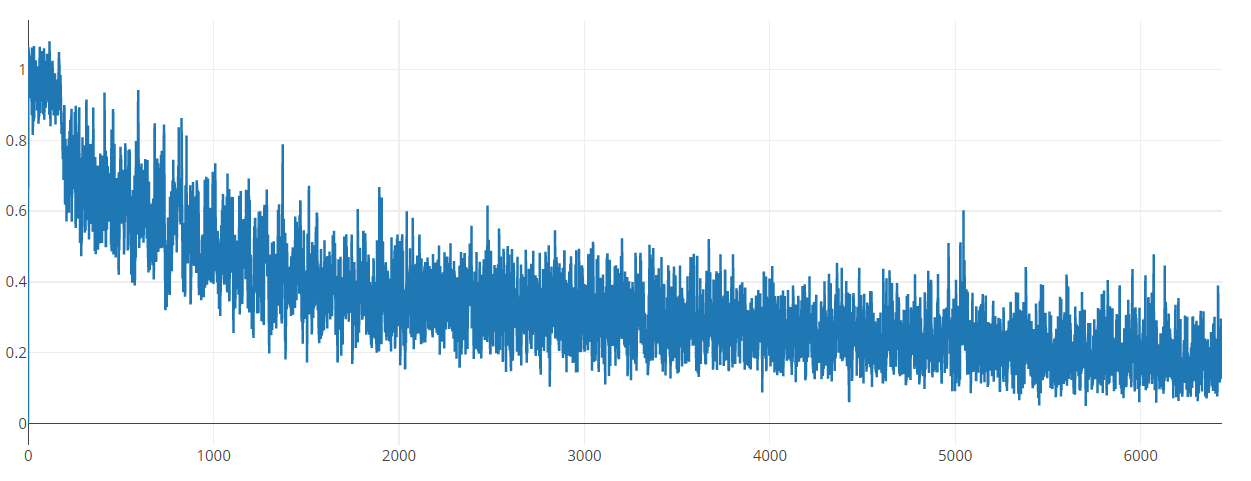
\includegraphics[width=0.5\textwidth]{p12.png}


\begin{thebibliography}{99}  
\bibitem{ref1} Zhang L, Wang S, Liu B. Deep Learning for Sentiment Analysis : A Survey[J].2018.
\bibitem{ref2} Liu  B.  Sentiment  analysis:  mining  opinions,  sentiments,  and  emotions.  The  Cambridge  University  Press, 2015.
\bibitem{ref3}Li  Z,  Zhang Y,  Wei  Y,  Wu  Y, and Yang  Q.  End-to-end  adversarial  memory  network  forcross-domain sentiment  classification.  In Proceedings  of  the  International  Joint  Conference  on  Artificial  Intelligence  (IJCAI 2017), 2017.  
\bibitem{ref4}Wang J , Yu L C , Lai K R , et al. Investigating Dynamic Routing in Tree-Structured LSTM for Sentiment Analysis[C] Conference on Empirical Methods in Natural Language Processing & International Joint Conference on Natural Language Processing. 2019.
\bibitem{ref5} Hu,Mengting.;Zhao,Shiwan.;Zhang Li.;CAN: Constrained Attention Networks for Multi-Aspect Sentiment Analysis. 2019.

\bibitem{ref6} Li,Zheng.;Li,Xin.;Wei,Ying., etal. Transferable End-to-End Aspect-based Sentiment Analysis with Selective Adversarial Learning .2019
\end{thebibliography}



\end{document}
